In order to make comparisons even more fair , the code about the application's core and UI is shared between different solution's implementations. This subsection presents the shared code in details. Some parts of the shared code can change from one implementation to another in order to adapt to the solution. However, changes to this structure are kept minimal. And the same is for the UI. It uses the least widget and visual features possible. In the Figure \ref{fig:todo_app_shared_folder_structure} the shared folder's and file's structure is shown. Subsequent paragraphs exaplains how models, pages, components and the repository are implemented. 

		
		\begin{figure}[H]
		    \centering
		    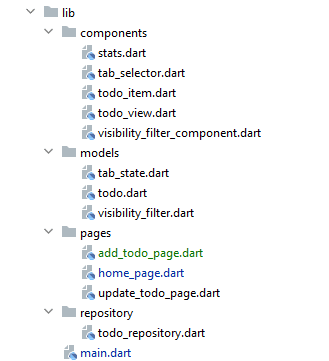
\includegraphics[width=0.6\textwidth]{Images/folder_structure.png}
		    \caption{Todos app skeleton's folders structure.}
		    \label{fig:todo_app_shared_folder_structure}
		\end{figure}
		
		
		
\paragraph{The application's Root} \mbox{} \\
		\label{par:todo_app_application_root}
The root widget of the application is called MyApp.
It is a stateful widget composed by a MaterialApp. Inside the MaterialApp, three routes are defined : the HomePage , the UpdateTodoPage and the AddTodoPage. The \textit{inizialRoute} is set to the HomePage as deafult. Inside the \textit{main} function the MyApp widget is passed to the \textit{runApp} method at the application's start.
		
		\mbox{}\\
		\captionof{listing}{Todo app - MaterialApp and main function definition} \mbox{}
	\begin{minted}{dart}
	
void main() {
  runApp(const MyApp());
}

class MyApp extends StatefulWidget {
  const MyApp({Key? key}) : super(key: key);

  @override
  State<MyApp> createState() => _MyAppState();
}

class _MyAppState extends State<MyApp> {

  @override
  Widget build(BuildContext context) {
    return MaterialApp(
      initialRoute: "/",
      routes: {
        "/": (context) => const HomePage(),
        "/updateTodo": (context) => UpdateTodoPage(),
        "/addTodo": (context) => AddTodoPage(),

      },
    );
  }
}

	
	\end{minted}
	\paragraph{Models and Repository} \mbox{} \\
	\label{par:todo_app_models_and_repository}
HomePage's tabs are only two : \textit{todos} and \textit{stats}. In the \textit{todos} tab todos are visualized. In the \textit{stats} tab ,instead, some numerical recap of the todos is visualized. They are defined using an enumeration for simplicity.

	\mbox{}\\
	
	\captionof{listing}{Todo app - TabState model definition}
	
	 \mbox{}
	\begin{minted}{dart}
	
	enum TabState{
	 todos,stats
	}
	
	
	\end{minted}
	
	\mbox{}
	
Filters for the \textit{filteredTodos} list are modelled by an enumeration too. They can take three values: \textit{all, notCompleted, completed}.
	
	\mbox{}\\
	
	\captionof{listing}{Todo app - VisibilityFilter model definition} \mbox{}
	\begin{minted}{dart}
	
	enum VisibilityFilter{
	 completed,notCompleted,all
	}
	
	
	\end{minted}
	
	\mbox{}
	
It's not possible to give a common implementation of the Todo model matching every solution. Todo model ,indeed, change in different implementations. The sharable structure of the model ,however, can defined as below RIFERIMENTO. (
	\mbox{}\\
	
	\captionof{listing}{Todo app - Todo model definitio} \mbox{}
	\begin{minted}{dart}
	
	@immutable
	class Todo {
	  final int id;
	  final String name;
	  final String description;
	  final bool completed;
	
	  const Todo(
	      {required this.id,
	      required this.name,
	      required this.description,
	      required this.completed});
	
	  @override
	  bool operator ==(Object other) {
	    return (other is Todo) &&
	        other.description == description &&
	        other.name == name &&
	        other.id == id &&
	        other.completed == completed;
	  }
	
	  @override
	  String toString() {
	    return "{ id: $id  completed: $completed}";
	  }
	
	  @override
	  // TODO: implement hashCode
	  int get hashCode => super.hashCode;
	}
	
	\end{minted}
	
	\mbox{}
	
	
The TodoRepository class simulate todos's fetching from a Database. It has two static methods. These methods are asynchronous and have a duration of 2 seconds to give the impression of a real asynchronous operation. The method \textit{loadTodos} , in particular , populate a list with six new todos after the generation of their unique ID's. Subsequently, after 2 seconds, returns it to the caller.
	
	\mbox{}\\
	
	\captionof{listing}{Todo app - TodoRepository definition} \mbox{}
	\begin{minted}{dart}
	
	class TodoRepository {
	  static Future<List<Todo>> loadTodos() async {
	    Random rand = Random();
	    List<Todo> todos = [];
	    List<int> ids = [];
	    while (ids.length < 6) {
	      int newInt = rand.nextInt(1000)+2;
	      if (!ids.contains(newInt)) {
	        ids.add(newInt);
	      }
	    }
	    todos = ids
	        .map((number) => Todo(
	            id: number,
	            name: "Todo " + number.toString(),
	            description: "description " + number.toString(),
	            completed: rand.nextBool()))
	        .toList();
	
	    await Future.delayed(const Duration(seconds: 2));
	    return todos;
	  }
	
	  static Future<void> saveTodos(List<Todo> todos) async {
	    await Future.delayed(const Duration(seconds: 2));
	  }
	}
	
	
	\end{minted}
	
	\mbox{}
	
	
	\paragraph{Pages} \mbox{} \\
	\label{par:todo_app_pages}
Homepage uses a simple Scaffold widget. The AppBar contains a VisibilityFilterComponent only when the tab is set to \textit{todos}. The body can change from \textit{todos} tab to \textit{stats} tab using the BottomNaviagationBar (the TabSelector). An empty FloatingActionButton is also present for future implementation.
	(note: some small pieces could change in different solution’s implementation. in the above example the tab changing is implemented through setState but it will not be always the case. Also ,the HomePage, can be muted to Stateless widget in other implementations.).
	
	\mbox{}\\
	
	\captionof{listing}{Todo app - HomePage definition} \mbox{}
	\begin{minted}{dart}
	class HomePage extends StatefulWidget {
	  const HomePage({Key? key}) : super(key: key);
	
	  @override
	  State<HomePage> createState() => _HomePageState();
	}
	
	class _HomePageState extends State<HomePage> {
	  TabState tab = TabState.todos; 
	
	  @override
	  Widget build(BuildContext context) {
	    return Scaffold(
	          appBar: AppBar(
	            actions: [
	              tab == TabState.todos
	                  ? const VisibilityFilterComponent()
	                  : Container()
	            ],
	            title: const Text("Todo App"),
	          ),
	          body: tab == TabState.todos ? const TodoView() : const Stats(),
	          bottomNavigationBar: TabSelector(
	            currTab: tab,
	            onTabChange:,
	          ),
	          floatingActionButton: tab == TabState.todos
	              ? FloatingActionButton(
	                  child: const Icon(Icons.plus_one),
	            onPressed: () {},
	          ) : null,
	        )
	    );
	  }
	}
	
	
	\end{minted}
	
	\mbox{}
	
	
	The UpdateTodoPage uses a Scaffold widget. The body is filled with a Column with two TextFields and a TextButton inside. The TextButton is left empty for future implementation.
	
	\mbox{}\\
	
	\captionof{listing}{Todo app - UpdatePage definition} \mbox{}
	\begin{minted}{dart}
	
	class UpdateTodoPage extends StatefulWidget {
	  final Todo todo;
	  final void Function(String,String) callback;
	
	  const UpdateTodoPage({Key? key, required this.todo,required this.callback}) : super(key: key);
	
	  @override
	  State<UpdateTodoPage> createState() => _UpdateTodoPageState();
	}
	
	class _UpdateTodoPageState extends State<UpdateTodoPage> {
	  final textControllerName = TextEditingController();
	  final textControllerDesc = TextEditingController();
	
	  @override
	  Widget build(BuildContext context) {
	
	    return Scaffold(
	        appBar: AppBar(
	          title: Text("Update Todo"+widget.todo.name),
	        ),
	        body: Column(
	          children: [
	            TextField(
	              controller: textControllerName,
	              decoration: const InputDecoration(
	                  border: OutlineInputBorder(), hintText: 'Enter a new name'),
	            ),
	            TextField(
	              controller: textControllerDesc,
	              decoration: const InputDecoration(
	                  border: OutlineInputBorder(), hintText: 'Enter a new description'),
	            ),
	            TextButton(onPressed: () {},
	            child: const Text("Confirm"))
	          ],
	        ));
	  }
	
	  @override
	  void dispose() {
	    textControllerName.dispose();
	    textControllerDesc.dispose();
	    super.dispose();
	  }
	}
	
	\end{minted}
	
	\mbox{}
	
	
	
	The AddTodoPage uses a Scaffold widget. The body is filled with Column with two TextField widgets and a TextButton widget inside. The TextButton is left empty for future implementation.
	
	\mbox{}\\
	
	\captionof{listing}{Todo app - AddTodoPage definition} \mbox{}
	\begin{minted}{dart}
	
	class AddTodoPage extends StatefulWidget {
	
	  final void Function(String,String) addTodoCallback;
	
	  const AddTodoPage({Key? key, required this.addTodoCallback}) : super(key: key);
	
	  @override
	  State<AddTodoPage> createState() => _AddTodoPageState();
	}
	
	class _AddTodoPageState extends State<AddTodoPage> {
	  final textControllerName = TextEditingController();
	  final textControllerDesc = TextEditingController();
	
	  @override
	  Widget build(BuildContext context) {
	
	    return Scaffold(
	        appBar: AppBar(
	          title: const Text("Add Todo"),
	        ),
	        body: Column(
	          children: [
	            TextField(
	              controller: textControllerName,
	              decoration: const InputDecoration(
	                  border: OutlineInputBorder(), hintText: 'Enter a name'),
	            ),
	            TextField(
	              controller: textControllerDesc,
	              decoration: const InputDecoration(
	                  border: OutlineInputBorder(), hintText: 'Enter a description'),
	            ),
	            TextButton(onPressed: () {}
	            , child: const Text("Create"))
	          ],
	        ));
	  }
	
	  @override
	  void dispose() {
	    textControllerName.dispose();
	    textControllerDesc.dispose();
	    super.dispose();
	  }
	}
	
	\end{minted}
	
	\mbox{}
	
	
	\paragraph{Components} \mbox{} \\
	\label{par:todo_app_components}
	Components are widgets created with a specific aims.
	TodoView component take care to visualize a list of todos. Todos are accessed in different ways depending on the implementation. TodoView uses a ListView widget. \textit{itemCount} and \textit{itemBuilder} fields are left empty for future implementation.
	
	\mbox{}\\
	
	\captionof{listing}{Todo app - TodoView definition} \mbox{}
	\begin{minted}{dart}
	class TodoView extends StatelessWidget {
	
	  const TodoView({Key? key}) : super(key: key);
	
	  @override
	  Widget build(BuildContext context) {
	    print("Building TodoView");
	
	
	    return ListView.builder(
	      itemCount:,
	      itemBuilder: (context, index) {
	        return TodoItem(
	          
	        );
	      },
	    );
	  }
	}
	
	\end{minted}
	
	\mbox{}
	
	
	TodoItem is a component that take care to visualize a specific todo. TodoItem is a stateless widget. It uses two Text widgets to display the todo's information and a Checkbox to change the todo’s completion. It is wrapped in a InkWell widget to make is responsive to taps. Functions are left empty for future implementation.
	
	\mbox{}\\
	
	\captionof{listing}{Todo app - TodoItem definition} \mbox{}
	\begin{minted}{dart}
	class TodoItem extends StatelessWidget {
	  final Todo todo;
	
	  const TodoItem({Key? key, required this.id}) : super(key: key);
	
	  @override
	  Widget build(BuildContext context) {
	    print("Building Todo Item \$todo");
	
	    return InkWell(
	      onTap: () {
	        Navigator.pushNamed(context, "/updateTodo");
	      },
	      child: Row(
	        children: [
	          Column(
	            children: [
	              Text(todo.name,
	                  style: const TextStyle(fontSize: 14, color: Colors.black)),
	              Text(todo.description,
	                  style: const TextStyle(fontSize: 10, color: Colors.grey)),
	            ],
	          ),
	          Checkbox(
	              value: todo.completed,
	              onChanged: (value) {}),
	        ],
	      ),
	    );
	  }
	}
	
	\end{minted}
	
	\mbox{}
	
	
	TabSelector component provides a way to switch from tabs. Tabselector uses a BottomNavigationBar with as many BottomNavigationBarItems as TabState.values (in our case two). Functions's fields are left empty for future implementation.
	
	\mbox{}\\
	
	\captionof{listing}{Todo app - TabSelector definition} \mbox{}
	\begin{minted}{dart}
	class TabSelector extends StatelessWidget {
	
	
	  const TabSelector(
	      {Key? Key})
	      : super(key: key);
	
	  @override
	  Widget build(BuildContext context) {
	    print("Building Tab Selector");
	
	    return BottomNavigationBar(
	      currentIndex: ,
	      onTap: (){},
	      items: TabState.values
	          .map((tab) => BottomNavigationBarItem(
	                label: describeEnum(tab),
	                icon: Icon(
	                  tab == TabState.todos ? Icons.list : Icons.show_chart,
	                ),
	              ))
	          .toList(),
	    );
	  }
	}
	
	\end{minted}
	
	\mbox{}
	
	VisibilityFilterComponent uses a DropdownButton with as many DropdownMenuItems as VisibilityFilter.values (in our case three). Function fields are left empty for future implementation.
	
	\mbox{}\\
	
	\captionof{listing}{Todo app - VisibilityFilterSelector definition} \mbox{}
	\begin{minted}{dart}
	class VisibilityFilterComponent extends StatelessWidget {
	
	  const VisibilityFilterComponent(
	      {Key? key})
	      : super(key: key);
	
	  @override
	  Widget build(BuildContext context) {
	    print("Building Visibility filter");
	    return DropdownButton<VisibilityFilter>(
	      value:,
	      items: VisibilityFilter.values.map((filter) {
	        return DropdownMenuItem<VisibilityFilter>(
	            child: Text(describeEnum(filter)), value: filter);
	      }).toList(),
	      onChanged: (filter) {
	       
	      },
	    );
	  }
	}
	\end{minted}
	
	\mbox{}
	
	Stats component takes care to visualize some numerical representation of the list of todos. Stats component is a Stateless widget composed by Text widget showing stats value.
	
	\mbox{}\\
	
	\captionof{listing}{Todo app - Stats definition} \mbox{}
	\begin{minted}{dart}
	class Stats extends StatelessWidget {
	  const Stats({Key? key}) : super(key: key);
	
	  @override
	  Widget build(BuildContext context) {
	    print("Building Stats");
	
	    return Text();
	  }
	}
	\end{minted}
	
	\mbox{}
	
	
